\part{Synthesis}
	\chapter{Introduction}
	Now that the relevant product fields are understood to a sufficient degree and the product's needs have been established we can begin to plan out how we will achieve the project's objectives. First we will established the methological approach that will structure the product's development. Then, for each of the core product requirements we will look at a high level design overview of how the requirement will be met, the actual implementation of this design, and testing to evaluate how well this requirement has been satisfied by this implementation.
	
	\chapter{Methological Approach}
	The project employed a prototyping methodology for development. First, we must perform an investigation into the system requirements, which was performed in the analysis with a list of specific core requirements being outlined in the conclusion. Following this the first prototype is built, which will resemble an incredibly basic scaled down version of how the final system should ideally look. This prototype is then thoroughly evaluated, with potential changes that would bring the prototype closer to the final system being figured out. Finally, these changes are then implemented and the prototype is evaluated once again. This is repeated until the product has reached its ultimate goals.
	
	%prototyping diagram?
	
	This methodology was employed partially due to the hardware nature of the product. Key features of the robot hinged on aspects like movement and observation being possible, so it was important to get a prototype that has this basic functionality up and working and quickly as possible. The prototyping approach allowed a pure focus on getting these functions working, and once they were the robot could be improved iteratively.
	
		\subsection{Initial Prototype}
		As previously stated, this methodology involves an initial prototype that all future prototypes will be an iteration of. The initial prototype of the project will involve the basic, primary construction of the robot. This will first involve the basic chassis assembly, followed by connecting relevant components to each other and then ensuring that they are all powered. Once this is done, we'll hopefully have an incredibly crude robot that won't be capable of much, but should hopefully serve as a solid foundation for future development toward the project goals.
		
		A similar approach will be followed for processing the map data. It won't be developed simultaneously at first as the robot needs to be capable of storing observational data from the LIDAR before the program can actually do anything, however it will start to be put together once the robot crosses this developmental threshhold.
	
	\chapter{Design}
	Before implementation of the specific project aims can be implemented, we first need the initial prototype that we can begin iteratively improving. Therefore, it's logical to design the initial robotic prototype first. What follows is an overview of how the initial robot prototype will be designed, followed by a breakdown of each of the individual project aims will be met.
	
		\section{Initial Prototype}
		Here will be the design for the base robot. The aim here is to achieve a solid foundation that all development can build on in order to meet the project objectives.
			\subsection{Hardware}
				\subsubsection{Chassis}
				First off will be the basic assembly of the three wheeled omnidirectional chassis. The chassis is comprised of two triangular metal plates, joined together by metal rods that are screwed into pre drilled holes that line up to eachother. The lower platform is where the motors and mounting points for the omnidirectional wheels are found, so once the plates have been connected the wheels will be pushed onto these mounting points and locked into place.
				% assembly diagram here?
				
				Now it's time for the microcontroller setup. The microcontroller used in this project is the FRDM-K64F, chosen for it's relatively low cost, small form factor and compatibility with the Micro C Operating System which is being employed for the robot's core program. To control the robot we'll also need a motor driver. The dfRobot Quad Motor Driver Shield is being employed for this project, it can be obtained from Amazon for around £13. It was chosen for this relatively low cost, the easily available documentation and the fact that it can easily plug into the FRDM-K64F, the microcontroller of choice for this project. The specifics behind how the shield will be used will be discussed during the movement design section, but in short it allows us to manipulate the energy being sent to the individual wheel motors which will afford us control over how they work and as such control over the robot's movement. Once these two components have been fitted together, the power and ground cables from each of the chassis motors will be plugged into the motor driver shield. Fig \ref{fig:shieldsetup} from the shield's documentation shows an example of this setup with four motors.
				
				\begin{figure}[h]
					\centering
					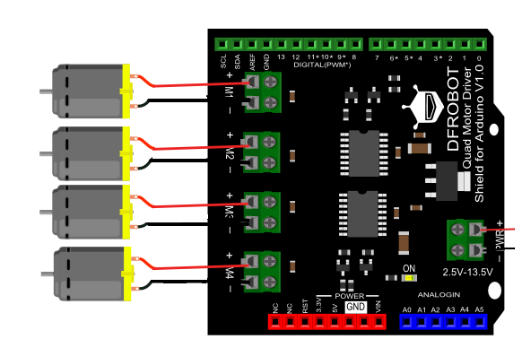
\includegraphics[width=.7\linewidth]{SYNTHESIS/shield_connection.png}
					\caption{Example shield setup}
					\label{fig:shieldsetup}
				\end{figure}
				
				The assembly shouldn't be overly complex, no soldering should be needed to connect components so it should be mostly a case of fitting things together.
				% explain LIDAR later.... :(
				
				\subsubsection{Power}
				The hardware components that will need powering are the three motors used to drive the omnidirectional wheels, the microcontroller, and the LIDAR sensor. The LIDAR sensor has two seperate pins that require power, one powering the motors that drives the LIDAR sensor and the other being the actual range finder itself. Table \ref{table:1} has a run down of these hardware components and the voltages that they use.
				
				\begin{table}[h!]
					\centering
					\begin{tabular}{|| l | l ||} 
						\hline
						Component & Voltage \\ [0.5ex] 
						\hline
						3x DC Coreless Motor  & 12V  \\ 
						FRDM-K64F  & 1.71 to 3.6V   \\
						RPLIDAR Scanner  & 5 to 5.5V  \\
						RPLIDAR Motor & 5 to 10V  \\ [1ex] 
						\hline
					\end{tabular}
					\caption{Components and respective voltages}
					\label{table:1}
				\end{table}
				
				To save on cost and complexity, it would be ideal to only use a single battery for the robot's power source. A single power source will be used for the robot, a battery holder containing 8 1.5V batteries will give us the 12V we need for the motors. Then, a step down voltage regular will be used to lower the voltage required for the other components. Fig \ref{fig:powersetup} has an overview of this.
				% !!!!!!!!!!!!!!!!!!!!!!!COME BACK TO THIS!!!!!!!!!!!!!!!!
			
			\subsection{Software}
			The software for the actual robot will be written in C++, compiled and deployed onto the microcontroller with the mbed SDK. At its foundation, it will be a Micro C OS with a series of configured tasks to perform various aspects of the robot's functionality. As you would expect, these tasks will come with their own memory tasks and will be designated with appropriate priorities. For the initial setup, we only need to make a skeleton OS to ensure we can properly compile and deploy code onto the microcontroller. Some relevant data structures and variables for task priorities and memory stacks, as well as a single task that prints hello world would be fine for this.
		
		\section{Designing for Requirements}
		Once this incredibly basic initial prototype is in place, we can begin to move toward truly fulfilling the project requirements. What follows is an overview of how each of the different project requirements will be met, with appropriate explanations toward the hardware and software employed.
		
			\subsection{Movement}
			The first of the three product aims outlined in the Analysis is that 'the robot must be capable of movement'.
				\subsubsection{Hardware}
				The previously mentioned dfRobot Quad Motor Driver Shield comes into play here. As shown in fig \ref{fig:shieldsetup}, the motors power and ground cables will connect to the appropriate pins on the shield. The motors can be manipulated once they receive power in this fashion. The shield is able to affect the electricity being sent to the motors by changing its polarity and by using pulse width modularity. By changing the pin to HIGH or LOW, we can affect the direction that the motor spins in (forward or backwards) and pulse width modulation allows us to affect the speed of the motor.
				
				\subsubsection{Software}
				In order to manipulate the motors we'll need some appropriate variables we can use to refer to the pins that the motor power and ground cables are connected to. %talk about pin lineup here and declaration
				
				% COME BACK TO THIS, TRIGONOMICAL NAVIGATION!

				
			\subsection{Observation}
				\subsubsection{Hardware}
				Only one range finder is being used to gather the observation data, the RPLIDAR A1M8 LIDAR sensor. The sensor is composed of a platform with a motor system that spins the range scanner as it takes readings, as well as some pins that can be used for communication. Fig \ref{fig:rplidarconfig} illustrates these components.
				
				\begin{figure}[h]
					\centering
					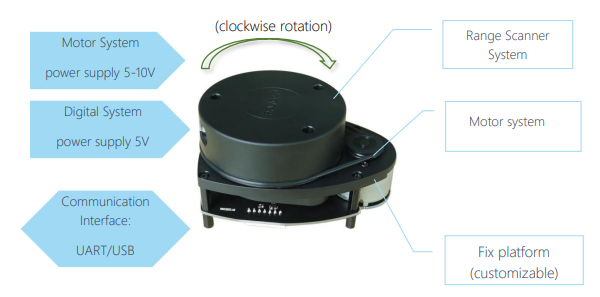
\includegraphics[width=.9\linewidth]{SYNTHESIS/rplidar_configuration.png}
					\caption{Example shield setup}
					\label{fig:rplidarconfig}
				\end{figure}
				
				\subsubsection{Software}
			\subsection{Processing Observational Data}
	
	\section{Designing for Requirements}
	%mention encoders?
		\subsection{Movement}
			
			\subsubsection{Hardware}
			\subsubsection{Software}		
			
		For this, the three wheeled omni directional chassis will be employed. This chassis was chosen due to the reduced cost compared to most other available chassis, and the omnidirectional wheels were ideal as the holonomic properties of the robot will allow it to move in any direction from any position without the need to first change its heading. To control the motors that will drive the wheels, the FRDM K64F MBED microcontroller will be used. The board is small, relatively cheap and will support the Micro-C Operating System that is going to be used as a structure for the robot's program. The motor driver
			
		From this, the robot will achieve an ability to move around an environment using basic navigation and the first of our three objectives will be met.
			
		\subsection{Observation}
		The second of the three product aims is that 'the robot must be capable of observation'.
			
		The RPLIDAR A1M8 360 Degree Laser Scanner will be used for the range finding aspect of this. Chosen for its high scan frequency and readily available SDK, it will be connected to the appropriate microcontroller pins so that it can recieve power and exchange information over a serial connection.
			
		This will allow the microcontroller access to range finding data and make it capable of utilizing the LIDAR sensor to observe the environment. A successful implementation here will achieve the second of our three product objectives.
			
		\subsection{Processing Observational Data}
		The last of the three product objectives is that 'the robot must be capable of processing observational data'.
		
		The plan for this is to use the CSM software described in the Analysis to process the robot's observational data. Once the robot has taken its observations, they will be saved onto an SD card that has been plugged into the FRDM K64F microcontroller. These observations will then be plugged into a computer where a created program will (once the user has directed it to) load this data and feed it into the CSM software. Once CSM has output an appropriate map, the program will display this to the user.
		
		Following a successful implementation of the above procedure, we will be capable of taking observational data and processing it into a viewable map. This will satisfy the last of the three project requirements.
	
	\medskip
	Now that we have a high level understanding of how each of the project objectives will be met, there will be a more thorough planning of how each of the hardware and software components will be implemented.
	
	% QUESTION - Should I discuss the cost of things here?
	\section{Hardware}
	This section aims to outline the hardware components selected for the project and to describe in a more detailed manner how the robot itself will be constructed.
	
		\subsection{Chassis}
			\subsubsection{Structure}
			The chassis is made up of an upper and a lower triangular platform, connected by small metal rods that screw into pre-drilled holes on the platforms. The lower platform features three 12 volt motors as well as mounting points for the omnidirectional wheels, which should lock into place once they are pressed onto it. %!! PUT ASSEMBLY DIAGRAM HERE?
			The space between the two platforms is where the robot's microcontroller and power supply will be housed, and the bulk of any wiring that needs to be done should ideally be here as well. On top of the upper chassis platform will be the LIDAR sensor used for range finding. It's important that the top platform remain relatively clean, as components or wiring being too close to the LIDAR may block the light it sends out and cause issues with the range finding process.
			
			The assembly shouldn't be overly complex, no soldering should be needed to connect components so it should be mostly a case of fitting things together.
			
			
			
		\subsection{Microcontroller}
			\subsubsection{FRDM-K64F}
			The FRDM-K64F will be employed to be the 'brain' of the robot. It's small, relatively cheap and compatible with the Micro C operating system which will run the tasks needed to be used for the robot's operation. As well, the freely available mbed SDK used for developing on these boards will make changing and redeploying code onto microcontroller quick and easy, which will help minimize time spent programming the next prototype iteration.
			
			\subsubsection{dfRobot Quad DC Motor Driver Shield}
			To manipulate the robot the way we want, we cannot simply supply all the wheels with full power all the time. This will make them constantly spin at the maximum rate. Omnidirectional navigation relies on having different wheels spin in different directions, often at different speeds. To achieve this, the motor driver shield will sit on top of our microcontroller. It features pins for each of the chassis motor's power and ground cables, and once plugged in we can run code on the microcontroller to change whether these pins are HIGH and LOW as well as the pulse width modulation of these pins. It was chosen for its ease of use and available documentation, as well as its immediate compatibility with the FRDM-K64F, installation will be as easy as plugged it into the board's GPIO pins. This will allow us to change both the direction and the speed of each of the individual wheels, which will help us achieve our omnidirectional navigation.
		
		\subsection{Sensor}
		The RPLIDAR A1M8 sensor will sit on top of the chassis and will be connected to the microcontroller. The microcontroller will provide the LIDAR with power, and a serial connection between the two components will allow the microcontroller to send and recieve information from the sensor. As mentioned in the power section, the LIDAR features two different pins that require power. These are the LIDAR motor and the LIDAR core, and they will recieve power that has been stepped down from the 12V battery pack that is being used.
	
	\section{Software}
		\subsection{Robot}
		The software for the actual robot will be written in C++, compiled and deployed onto the microcontroller with the mbed SDK. At its foundation, it will be a Micro C OS with a series of configured tasks to perform various aspects of the robot's functionality. As you would expect, these tasks will come with their own memory tasks and will be designated with appropriate priorities.
		
			\subsubsection{Sensor}
			In order to interface with the RPLIDAR A1M8, SLAMTEC's own SDK will be used. The SDK comes in the form of header files which appropriately implement the functionality needed to send requests and recieve information from the LIDAR sensor. Table \ref{table:3} has a manifest of the SDK and the functionality that it provides.
			
			\begin{table}[h!]
				\centering
				\begin{tabular}{|| l | l ||} 
					\hline
					File & Purpose \\ [0.5ex] 
					\hline
					rplidar.h  & Parent file for subsequent header files  \\ 
					rplidar\textunderscore driver.h  & Provides RPLidarDriver class for  interfacing with sensor   \\
					rplidar\textunderscore  protocol.h  & Defines structs and constants for the LIDAR protocol  \\
					rplidar\textunderscore  cmd.h & Defines request/answer structs for LIDAR protocol  \\ 
					rptypes.h & Platform independent structs and constants  \\ [1ex] 
					\hline
				\end{tabular}
				\caption{RPLIDAR SDK files}
				\label{table:3}
			\end{table}
		
		
		\subsection{Map Building}
	
		\subsubsection{FRDM-K64F}
		The FRDM-K64F will be employed to be the 'brain' of the robot. It's small, relatively cheap and compatible with the Micro C operating system which will run the tasks needed to be used for the robot's operation. As well, the freely available mbed SDK used for developing on these boards will make changing and redeploying code onto microcontroller quick and easy, which will help minimize time spent programming the next prototype iteration.
	
		\subsection{Sensor}
		The RPLIDAR A1M8 sensor will sit on top of the chassis and will send data to the microcontroller over a serial connection. Once this connection has been established, the microcontroller will be able to send request to the LIDAR. An overview of the possible requests that can be sent to the LIDAR can be seen in table \ref{table:2}.
		
		\begin{table}[h!]
			\centering
			\begin{tabular}{|| l | l ||} 
				\hline
				Function & Purpose  \\ [0.5ex] 
				\hline
				Scan & Begin scanning  \\ 
				Stop & Stop scanning  \\
				Reset & Reboot RPLIDAR core  \\
				Force Scan & Begin scanning without checking rotation speed  \\
				Get Info & Output device info (e.g. serial number)  \\
				Get Health & Output device health info  \\
				Get Samplerate & Output single sampling time  \\
				Get Lidar Conf & Get LIDAR configuration  \\ [1ex] 
				\hline
			\end{tabular}
			\caption{RPLIDAR SDK overview}
			\label{table:2}
		\end{table}
		

		
	\chapter{Implementation}
	\chapter{Testing}